\nnarticleheader{Putting a Spin on the Average Bike}{Jaiden Shuchman, Jay Crowther, and Ryan Davey, Haverford '23}
In 2018, Denise Mueller-Korenek rode a bicycle at 183.9 mph, shattering the previous world record set by Fred Rompelberg, which was 166 mph. Mueller-Korenek accomplished this not only by riding in the slipstream of a drag racer, but by using a custom bike.  Mueller-Korenek’s bike contained extra gears. These gears allowed her to reach her incredible record-breaking speeds. Mueller-Korenek’s unique bike led us to the question: how much do  extra gears affect the speed at which the tires rotate?

Immediately, we understood that a combination of the gears, rpm of the wheels, and the size of the wheels would determine the speed of the bicycle. Investigating this concept presented  many challenges, so we decided to explore only two variables: the number of gear systems and  the ratio of the cog sizes. These values would affect the rpm of the wheels. The speed was not part of our investigation, however, by using the size of the wheels as well as the rpm, velocity  was easily calculated. We used the dimensions of Mueller-Korenek’s bicycle to find the increase in rpm to the bicycle with the addition of more gear systems. We were forced to make logical assumptions for some dimensions of the bike because they were not provided. The image to the left is our quick sketch of the additional gear systems and features a chart to record the top  speeds from the different systems. 

Once we established our main hypothesis, that the addition of gears would increase the rpm of the wheels linearly, we began the mathematical portion of the project. The first step was to figure out the angular velocity and overall metrics of the bike used by Mueller-Korenek.

The equation for angular velocity is the amount of revolutions divided by the time, measured in revolutions per minute. First, knowing that the diameter of the tire was equal to 17 inches, we deduced that the radius would be half that: 8.5 inches. By using the equation for circumference, $C=2 \pi r$, we found that the distance traveled in a full revolution of the tire is roughly 53.4 inches, or $17\pi$ inches. Mueller-Korenek traveled a maximum speed of 183.9 mph, and there are 63360 inches in a mile. With this information, we then multiplied 63,360 by 183.9 to get approximately 11,651,904, which is Mueller-Korenek’s speed converted to inches per hour. We can now divide this by the circumference of the wheel to get the revolutions per hour and we get about 218,200 revolutions per hour. Divide this by 60 to get around 3,638  revolutions per minute.\footnote{Alternate Method: $184=17 \pi r$; $r$ equals revolutions, and 17$\pi$ is the circumference of the wheel. 184 is the maximum speed of the bike. In this equation, you find the number of revolutions in a single hour. By converting the 184 miles into feet, and the 17$\pi$ inches into feet, you are left with $971520=4.4505r$. Then solve for $r$. The following number is the rotations per hour. Divide by 60 to find the rpm, which is 3638.}

$$
\frac{183.9 \text{ mi}}{\text{ hr}} \times \frac{63,360 \text{ in}}{\text{ mi}} \times \frac{1 \text{ rev}}{17\pi \text{ in}} \times \frac{1 \text{ hr}}{60 \text{ min}} = 3,638 \text{ rpm}
$$

The bike tire is attached by an axle to a 12 cog wheel which in turn is connected to a 60 cog wheel by a 55 inch chain.\footnote{This is also an approximation from an average bicycle}
The ratio of 12 to 60 is equivalent to a 1 to 5 ratio. Therefore, we can divide the amount of revolutions by 5 to get the rpm of the 60 cog wheel because it will have to travel 5 times the distance of the chain to accomplish 1 full revolution. 

At Mueller-Korenek’s maximum velocity of 183.9 mph, the 60 cog wheel will be moving at a rate of 727.6 rpm. However, that 60 cog wheel is connected by another axle to a 12 cog wheel, which in turn is connected by a 55 inch chain to another 60 cog wheel.\footnote{This is also assumed.} 
We can do the same math as above, by finding the ratio of 12 to 60 and then dividing, and we get approximately 145.52 rpm for that final 60 cog wheel at Mueller-Korenek’s max speed. That 60 cog wheel is connected directly to the pedals, meaning that she is pedaling at an average of 145.52 rpm. For every time she pedals, her back wheel is turning approximately 25 times.

\begin{align*}
\frac{60}{12} &= 5 \\
\frac{727.6 \text{ rpm}}{5} &= 145.52 \text{ rpm} 
\end{align*}

As we know based on our data, each additional cog with a 60 to 12 ratio yields approximately 5 times as many revolutions per minute of the tires. This is an exponential increase which is proportional to the number of cogs added (starting from 0 gears). This can be modeled after $5^{x}$ because each successive cog will multiply the speed by 5. The equation of this function is $y=145.52(5^{x})$,\footnote{https://www.desmos.com/calculator/opplgoh8i1} where the amount of gear systems with the pedals themselves being 0 is equal to $x$. We are assuming that she is pedaling at a constant speed of 145.52 rpm. From this graph we can determine that when $x$ equals 0, $y$ equals 145.52. When $x = 1$, $y$ should be equal to roughly 727.6. When $x = 2$, $y$ should be going at roughly 3638. When $x = 3$, $y$ should  be roughly 18190 rpm. 

\begin{align*}
145.52(5^{0}) &= 145.52(1) \\
&= 145.52 \text{ rpm} \\
\end{align*}

\vspace{-10mm}

\begin{align*}
145.52(5^{1}) &= 145.52(5) \\
&= 727.6 \text{ rpm} \\
\end{align*}

\vspace{-10mm}

\begin{align*}
145.52(5^{2}) &= 145.52(25) \\ 
&= 3638 \text{ rpm} \\
\end{align*}

\vspace{-10mm}

\begin{align*}
145.52(5^{3}) &= 145.52(125) \\
&= 18,190 \text{ rpm}
\end{align*}

\vspace{5mm}

\renewcommand{\thefigure}{1}
\begin{figure}[h]
    \centering
    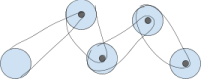
\includegraphics{gears.png}
    \caption{The overall gear pattern at $x=4$}
\end{figure}

If the wheel is connected to the final gear in the sequence, it will be traveling at 90950 rpm, or 4600mph. However, this is pretty much impossible due to the issues of getting to this speed and the fact that no human body or bicycle can withstand this velocity.

Hypothetically, if the bike and rider are indestructible, how many gears do we need to reach the speed of light? The speed of light is 670,616,629 mph, which is equivalent to 13,261,632,213.93 rpm of the wheel with a $17\pi$ inch circumference. Assuming she is pedaling at the same constant speed of 145.52 rpm,  we plugged that very large number in for $y$, solved for $x$, and got 11.38771942. This number is the amount of groups of 60 tooth to 12 tooth gears with 55 inch chains (gear systems), needed to  reach the speed of light if she pedals at the speed she did when she reached 184 mph. Obviously, this is impossible for a number of reasons from friction, to the structural integrity of the bike and rider.  

$$
    \frac{670,616,629 \text{ mi}}{\text{ hr}} \times \frac{1 \text{ hr}}{60 \text{ min}} \times \frac{63,360 \text{ in}}{\text{mi}} \times \frac{1 \text{ rev}}{17\pi \text{ in}} = 13,261,632,213.93 \text{ rpm} \\
$$

\begin{align*}
    145.52(5^{x}) &= 13,261,632,213.93 \\
    5^{x} &= 91,132,711.75  \\
    x &= \log_5 91,132,711.75  \\
    x &= 11.38771942 \text{ gear systems}
\end{align*}

The equation $y=pn^{x}$ can be used to determine the rpm of a bike’s wheels that has a fixed ratio between gear sizes. $p$ is the amount of revolutions per minute of the pedals, $n$ is the ratio of the gears, $x$ is the amount of gear systems, and $y$ is the revolutions per minute of
the wheel. If you multiply $y$ by whatever the circumference of the wheel is, you get the speed of the bike.  

We arrived at this function through a series of logical steps using the data and  dimensions of the initial bike used by Mueller-Koerner. We observed that the wheel attached to  the pedals, or in terms of our equation $x=0$, is spinning at 145.52 rpm.  Therefore, $y=145.52$ rpm. Following this discovery for the first gear system, the gear was spinning at 727.6 rpm, a jump by 5 times greater than the previous value. The wheel itself was spinning at roughly 3638 rpm, which once again, is 5 times faster than the previous gear. This showed us that each gear roughly had a 1:5 ratio with the successive gear; at this point, we realized that this meant each consecutive gear multiplied the previous gear’s speed by 5, so this meant it could be modeled by a transformation of the function $5^{x}$. Now, using prior knowledge, we understood that when $x=0$, the $y$-value had to be equal to 145.52. This is the rpm of the pedals initially. We then determined that the only way to achieve this with a transformation  of our function was to multiply $5^{x}$ by this number, leaving us with the equation $145.52(5^{x})$. From this, we can determine that the number multiplied by $5^{x}$ (which is denoted by the variable $p$) is always the amount of revolutions per minute of the pedals (essentially, this is the angular velocity  of the first gear). Also, we can confirm that the base 5 (denoted by $n$ in our equation) is the ratio  from each gear to the successive one, making $n$ the growth factor for the speed.  
From this equation, we can see that it is theoretically possible, with an indestructible bike and a sufficient force to pedal the bike and hold itself together, it is possible to go infinitely fast.  We multiply the output of the wheels by 5 every time a gear system is added (in the event that the gear system is the same as Mueller-Korenek’s), so it is an exponential growth. 

To further prove the validity and accuracy of our function, we used the dimensions from another familiar bike: Mr. Bridge’s 20 speed bike. All of these calculations were performed  assuming there is no outside force acting upon this bike when in motion (e.g. air resistance and  friction) and that Mr. Bridge is strong enough to pedal at any speed he pleases. The radius of the tires is 14 inches, therefore making the circumference $28\pi$ inches. Following this, we counted the teeth on each gear, resulting in the values 52 and 11 for their respective gears. We then calculated  the gear ratio (by dividing these numbers) to be approximately 4.7272. We now have enough  information to plug these values into our equation and set up the problem.  

We assumed that Mr. Bridge was pedaling at 100 rpm, a high number,  but as we stated previously, strength is no concern for Mr. Bridge. Our equation, with the inserted values, was $y=100(4.7272^{1})$: Mr. Bridge’s bike possessed only a single gear system,  so $x$ can be substituted with the value 1. After solving this equation, we get $y=472.72$ rpm.  If we multiply this number by the circumference of the wheel, that being $28\pi$ or 87.962, we can  find the linear velocity. This ended up being equal to 41581.4 inches per minute. We converted this to 2494883.8 inches per hour by multiplying the previous value by 60. Then, we divided this by 63360 (the number of inches in one mile) to get a value of 39.376 miles per hour.  This value is how fast Mr. Bridge would be going if he pedaled at an angular velocity of 100 rpm and was in the highest gear possible for his bike. This result is realistic and makes sense given that Mr. Bridge is unable to pedal 100 rpm in real life, so his real speed would be less based on air resistance, friction, and a lack of strength.  

\begin{align*}
y=100(4.7272^{1}) \\
= 472.72 \text{ rpm} 
\end{align*}

$$
\frac{472.72 \text{ rev}}{\text{min}} \times \frac{28\pi \text{ in}}{\text{rev}} \times \frac{60 \text{ min}}{\text{hr}} \times \frac{1 \text{ mi}}{63360 \text{ in}} = 39.376 \text{ mph}
$$

In reflection, we learned that our hypothesis, that if more gear systems were added then  the rpm of the bike would increase linearly, was wrong. It turned out that the addition of extra gear systems would result in an exponential increase in rpm. After watching the video of Californian biker Denise Mueller-Korenek breaking the world record of the top speed traveled on  a bike, we weren’t very moved. However, what caught our attention was the bike Mueller-Korenek used to do so. Seeing the extra gear systems on her bike we had a million  questions, most of which being ridiculous. One question that stuck though, was to what degree did the gears affect the speed of her bike? After our research we learned just how powerful the addition of extra gears are. It’s truly mind boggling when you see something so small have such  an insane amount of repercussions. Small things tend to make huge differences, whether you  expect it or not. 

\pagebreak

\noindent

\begin{thebibliography}{4}
\bibitem{openstax} 
“10.2 Kinematics of Rotational Motion - College Physics.” OpenStax,  
openstax.org/books/college-physics/pages/10-2-kinematics-of-rotational-motion.  

\bibitem{chappel}
Chappell, Bill. “Woman Rides Bicycle To 183.9 MPH - A World Record.” NPR, NPR, 18 Sept.  2018,  
www.npr.org/2018/09/18/649221471/woman-rides-bicycle-to-183-9-mph-a-new-world-record

\bibitem{stout}
Stout, James. “The Crazy Detail That Went Into Creating This Record-Breaking Bike.” Bicycling , Bicycling, 20 Sept. 2020,  
www.bicycling.com/bikes-gear/a23305843/what-went-into-creating-this-record-breaking-bike/

\bibitem{mbs}
“Table Of Radius Values For Bicycle Sprockets.” Machinehead Bike Software,  
\url{www.machinehead-software.co.uk/bike/chain_length/sprocket_radius_table.html}

\end{thebibliography}
